\documentclass[10pt,aspectratio=169]{beamer}

% All the boilerplate is in deslides.sty
\usepackage{deslides}

\author{Ji\v{r}\'i Lebl}

\institute[OSU]{%
Oklahoma State University%
%Departemento pri Matematiko de Oklahoma {\^S}tata Universitato%
}

\title{4. Integrals as solutions (Notes on Diffy Qs, 1.1)}

\date{}

\begin{document}

\begin{frame}
\titlepage

%\bigskip

\begin{center}
The textbook: \url{https://www.jirka.org/diffyqs/}
\end{center}
\end{frame}

\begin{frame}
Consider a general first order ODE:
\[
\frac{dy}{dx} = f(x,y) ,
\quad\text{or}\quad
y' = f(x,y) .
\]
\pause
There is no single, simple procedure where you turn a crank and out pops a
solution.

\medskip
\pause

In the case
\[
y' = f(x) ,
\]
\pause
antidifferentiate (integrate) both sides:
\[
\int y'(x) \,dx = \int f(x) \,dx + C ,
\quad\pause\text{or}\quad
y(x) = \int f(x) \,dx + C .
\]
\pause
That's the \emph{general solution}.

\medskip
\pause

\textbf{Example:}
Find the general solution of $y' = 3 x^2$.

\medskip
\pause

Integrate:\quad
$y = x^3 + C$.

\medskip
\pause

Check (differentiate):\quad
$y' = \pause 3x^2$.
\quad
{\Large\checkmark}
\end{frame}

\begin{frame}
Note that $\int f(x) \, dx$ means an antiderivative.

\medskip
\pause

An antiderivative can be computed via a definite integral:
\[
y(x) = \int_{x_0}^x f(t) \,dt + C .
\]
\pause
Even if there is no ``closed form'' answer, that gives you
an exact formula.

\medskip
\pause

Usually also an initial condition (IC) \quad $y(x_0) = y_0$.

\medskip
\pause

The solution to $y' = f(x)$, $y(x_0)=y_0$ is
\quad
$\displaystyle
y(x) = \int_{x_0}^x f(t) \,dt + y_0$.

\medskip
\pause

Is it a solution to the DE?
\pause
Yes by FTC!

\medskip
\pause

Does it satisfy the IC?
\quad
\pause
$\displaystyle y(x_0) = \pause \int_{x_0}^{x_0} f(t)\,dt + y_0 \pause = y_0$.
\quad
{\Large\checkmark}

\medskip
\pause

\textbf{Example:}
Solve
$y' = e^{-x^2}$, $y(0) = 1$.
\pause
\[
y(x) = \int_0^x e^{-t^2} \,dt + 1 .
\]
\end{frame}

\begin{frame}
So far, that's just regular Calc 1.

\medskip
\pause

How about \quad
$y' = f(y)$\quad ?

\medskip
\pause

Write it in the \emph{Leibniz notation}:
\quad
$\displaystyle
\frac{dy}{dx} = f(y)$.

\medskip
\pause

Inverse function theorem says:
\quad
$\displaystyle
\frac{dx}{dy} = \frac{1}{f(y)}$.

\medskip
\pause

Now integrate:
\quad
$\displaystyle
x(y) = \int \frac{1}{f(y)} \,dy + C$.

\medskip
\pause

What's wrong?
\pause
We have $x$ in terms of $y$, not $y$ in terms $x$.

\pause
\medskip

So solve for $y$!
\end{frame}

\begin{frame}
\textbf{Example:}
Let's use the method to solve $y'=ky$ ~~($k > 0$).

\medskip
\pause

Note that $y=0$ is a solution.

\medskip
\pause

Assume $y\not= 0$ and write
\quad$\displaystyle
\frac{dx}{dy} = \frac{1}{ky}$.

\medskip
\pause

Integrate:
\quad
\quad$\displaystyle
x(y) = x = \frac{1}{k} \ln \, \lvert y \rvert + D$,

\medskip

$D$ is an arbitrary constant.

\medskip
\pause

Solve for $y$:
\quad
\quad$\displaystyle
\lvert y \rvert =
e^{kx-kD} = 
e^{-kD} e^{k x}$.

\medskip
\pause

If we let $C$ be arbitrary, then $y=Ce^{kx}$ includes all
the possibilities, including $y=0$.
\end{frame}

\begin{frame}
\textbf{Example:}
Find the solution of
$y' = y^2$,~ $y(0)=1$.

\medskip
\pause

Note that $y=0$ is a solution, so we can now assume $y \not= 0$.

\medskip
\pause

Write:
\quad
$\displaystyle
\frac{dx}{dy} = \frac{1}{y^2}$.
\qquad
\pause
Integrate:
\quad
$\displaystyle
x = \frac{-1}{y} + C$.
\qquad
\pause
Solve for $y$:
\quad
$\displaystyle
y = \frac{1}{C-x}$.

\medskip
\pause

The general solution is
\quad
$\displaystyle
y = \frac{1}{C-x} \qquad \text{or} \qquad y = 0$.

\medskip
\pause

IC ~$y(0)=1$~ leads 
to $C=1$ or $y = \frac{1}{1-x}$.

\medskip
\pause

This solution has a singularity.

\medskip
\pause

$y$ ``blows up'' as $x\to 1$.

\vspace*{-0.7in}
\hspace*{2.5in}%
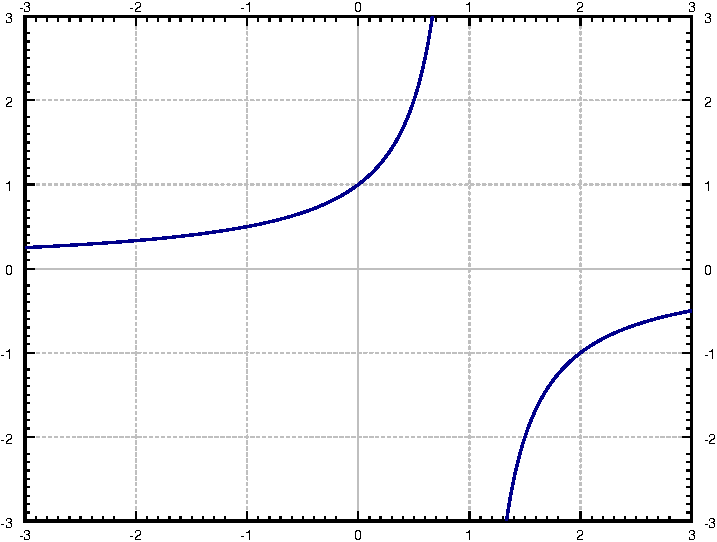
\includegraphics[height=1.9in]{../figures/1over1mx}

\vspace*{-1.15in}
\pause

$y'=y^2$ seems so nice,

yet $y$ is so badly behaved.

\medskip
\pause

$y$ is only defined on $(-\infty,1)$

\medskip
\pause

$(1,\infty)$, doesn't include our
IC.

\medskip
\pause

So the right hand side of the graph

isn't really part of our solution.
\end{frame}

\begin{frame}
Problems solvable by integration often deal
with \emph{velocity}, \emph{acceleration}, and \emph{distance}.

\medskip
\pause

\textbf{Example:}
A car drives at a speed of $e^{t/2}$ meters per second, where $t$ is time in seconds.

How far did the car get in 2 seconds (starting at $t=0$)?  How far in 10 seconds?

\medskip
\pause

Denote by $x$ the distance traveled.
\pause
Equation is \quad $x' = e^{t/2}$.

\medskip
\pause

General solution is: \quad
$x(t) = 2 e^{t/2} + C$.

\medskip
\pause

At $t=0$, $x=0$, so IC is:
\quad
$0 = x(0) \pause = 2e^{0/2} + C \pause = 2 + C$
\pause
\wthus
$C=-2$.

\medskip
\pause

Solution: 
\quad
$x(t) = 2 e^{t/2} - 2$.

\medskip
\pause

At 2 and 10 seconds we are at
\begin{equation*}
x(2) = 2e^{2/2} - 2 \approx 3.44 \text{ meters} ,
\pause
\qquad
x(10) = 2e^{10/2} - 2 \approx 294 \text{ meters} .
\end{equation*}
\end{frame}

\begin{frame}
\textbf{Example:}
Suppose that the car accelerates at $\unitfrac[t^2]{m}{s^2}$.
\pause
At time $t=0$ the car is at the 1 meter mark and is traveling at
\unitfrac[10]{m}{s}.
\pause
Where is the car at time $t=10$?

\medskip
\pause

Actually a second order problem.

\medskip
\pause

Let $x$ be the distance.
\quad
Then $x'$ is the velocity.
\quad
And $x''$ is the acceleration.

\medskip
\pause

The full problem: \quad $x'' = t^2 , \quad x(0) = 1 , \quad x'(0) = 10$.

\medskip
\pause

Give $x'$ a name, say $v=x'$.

\medskip
\pause

Then we have the subproblem: \quad 
$v' = t^2, \quad v(0) = 10$.

\medskip
\pause

So solve for $v$, then as $x'=v$ solve for $x$ by integration.

\pause

\begin{exercise}
Solve for $v$, and then solve for $x$.  Find $x(10)$ to answer the
question.
\end{exercise}

\end{frame}

\end{document}
